\documentclass[a4paper,10pt]{article}
%\documentclass[a4paper,10pt]{scrartcl}

\usepackage[utf8]{inputenc}
% The following packages can be found on http:\\www.ctan.org
\usepackage{graphics} % for pdf, bitmapped graphics files
\usepackage{graphicx}
%\usepackage{epsfig} % for postscript graphics files
\usepackage{mathptmx} % assumes new font selection scheme installed
\usepackage{times} % assumes new font selection scheme installed
\usepackage{amsmath} % assumes amsmath package installed
\usepackage{amssymb}  % assumes amsmath package installed
\usepackage{algorithm}
\usepackage{algorithmic}
\usepackage{authblk}
\usepackage{hyperref}
\usepackage{url}
% \usepackage{xfrac}
% \usepackage{helvet}
% \usepackage{arial}
% \DeclareMathOperator{\argmin}{\textit{argmin}}
\usepackage[retainorgcmds]{IEEEtrantools}

\title{Reference frames for {IMAV2013}}
\author{P, JL, JP}
\date{2013 August 25}

\pdfinfo{%
  /Title    ()
  /Author   ()
  /Creator  ()
  /Producer ()
  /Subject  ()
  /Keywords ()
}

\begin{document}
\maketitle

\begin{figure}[tbh!]
\centering
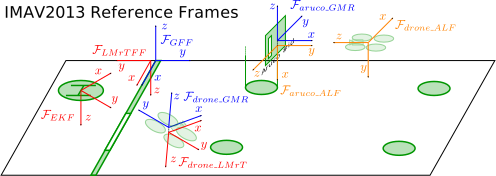
\includegraphics[width=1.0\columnwidth]{General_Frames_Field.pdf}
\caption{
	  These are the main reference frames used on our IMAV2013 code.
	  } \label{fig:IMAV_Frames}
\end{figure}

Reference frames acronyms, see Fig.~\ref{fig:IMAV_Frames}:
\begin{enumerate}
 \item GFF: Global Fixed Frame
 \item {EKF}, Extended Kalman Filter
 \item Frames fixed on the {ArUCo} codes:
 \begin{enumerate}
  \item aruco\_{GMR}, Ground Mobile Robotics
  \item aruco\_{ALF}, Aruco Library Frames
 \end{enumerate}
 \item Frames fixed on the drone's {COG}:
 \begin{enumerate}
  \item drone\_{GMR}
  \item drone\_{ALF}
  \item drone\_{LMrT}, Local Multirotor Telemetry (droneMsgs::droneNavData)
 \end{enumerate}
\end{enumerate}

We send the relative position between the above mentioned frames using a droneMsgs::dronePose message, which contains:
the translation vector $\{ x, y, z\}$; and the relative attitude codified in an YPR system $\{ yaw, \psi; pitch, \theta; roll, \phi\}$.
The message also specified the YPR convention (which is need to ensure that the rotation matrix $R$ is appopiately decodified),
the reference frame and the target frame. This information can be converted into a homogeneous transformation matrix to perform
the calculation:

$ \left[
  \begin{array}{c}
   p_{ref} \\
   1
  \end{array}
  \right]
  =
  \left[
  \begin{array}{cc}
   R & O_{ref}O_{target}\\
   0 & 1 
  \end{array} 
  \right]
  \cdot
  \left[
  \begin{array}{c}
   p_{rel} \\
   1
  \end{array}
  \right]
  =
  \left[
  ^{target}_{reference}T_{YPR convention}
  \right]
  \cdot
  \left[
  \begin{array}{c}
   p_{rel} \\
   1
  \end{array}
  \right]
  $

  \newpage
Used YPR convenctions:
\begin{enumerate}
 \item \textbf{wYvPuR}, this is our main convention which is used in {ROS} topics. which is equivalent to $xRyPzY$
 \item \textbf{xYyPzR}, which is equivalent to $wRvPuY$
 \item to understand equivalences, checkout: 
 \href{http://en.wikipedia.org/wiki/Euler\_angles\#Conversion\_between\_intrinsic\_and\_extrinsic\_rotations}{http://en.wikipedia.org/wiki/Euler\_angles\#Conversion\_between\_intrinsic\_and\_extrinsic\_rotations}
 \item to know how to perform the inverse mapping from rotation matrix to YPR values, checkout:
 \href{http://en.wikibooks.org/wiki/Robotics\_Kinematics\_and\_Dynamics/Description\_of\_Position\_and\_Orientation\#Inverse\_Mapping\_2}{http://en.wikibooks.org/wiki/Robotics\_Kinematics\_and\_Dynamics/Description\_of\_Position\_and\_Orientation\#Inverse\_Mapping\_2}
 \item note that:
 \begin{enumerate}
  \item $R_{wYvPuR} = R_{wY}R_{vP}R_{uR}$
  \item $R_{xYyRzR} = R_{xY}R_{yP}R_{zR}$
 \end{enumerate}
\end{enumerate}

Inicialization:
\begin{itemize}
 \item Configuration file giving an approximate location of the take off site.
 \item The yaw drift that occurs same time can be a problem: to address it we are going to use the initial value of the measured yaw to locate $\mathcal{F}_{EKF}$
\end{itemize}

Other things:
\begin{itemize}
 \item We are going to locate the {ArUCo} so that the YPR representation singularities are located above and below them.
 \item Unfortunately, not all the EKF estimations are correct. The ones that are reliable are: x, y, z, yaw, vx, vy, vmx, vmy.
 \item For the rest of the required estimations we will use the telemetry data directly
 \item Notat that the magnetometer does not always correct the yaw drift. This issue is present in both, EKF and telemetry data.
\end{itemize}

A graph showing the modules and the topics that are exchanged among them is shown on Fig.~\ref{fig:IMAV_Modules}.

\begin{figure}[tbh!]
\centering
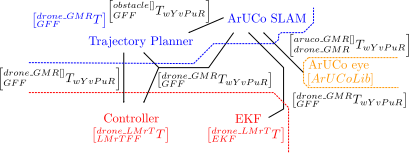
\includegraphics[width=0.70\columnwidth]{Module_communication_IMAV13.pdf}
\caption{
	  These are the main modules used on our IMAV2013 code. ROS topics are in black
	  } \label{fig:IMAV_Modules}
\end{figure}

\end{document}
